\section{Metodologia}
\label{sec:metodologia}

%O módulo \texttt{01\_\allowbreak analise\_\allowbreak socios} implementa um \textit{pipeline} determinístico em Python (\texttt{pandas}~\cite{mckinney2010pandas}, \texttt{numpy}, \texttt{networkx}~\cite{hagberg2008networkx} e \texttt{matplotlib}~\cite{hunter2007matplotlib}), orquestrado pelo utilitário \texttt{run\_\allowbreak pipeline\allowbreak .py} (\texttt{-{}-offline --with-graphs}) para execução em Linux e disponível em repositório público~\cite{projeto_github}. Sobre dados de Divinópolis/MG, o fluxo encadeia quatro módulos e consolida grafos \texttt{.gexf} no Gephi~\cite{bastian2009gephi} sob pseudonimização integral (Figura~\ref{fig:fluxograma_eixo1}): (1)~Higienização \& Grafo Base, (2)~Enriquecimento QSA \& Score, (3)~Redução \& Triângulos $K_3$, (4)~Materialidade \& Anti-FP e (5)~Grafos \texttt{.gexf} \& Achados LGPD.

\begin{figure*}[!t]
\centering
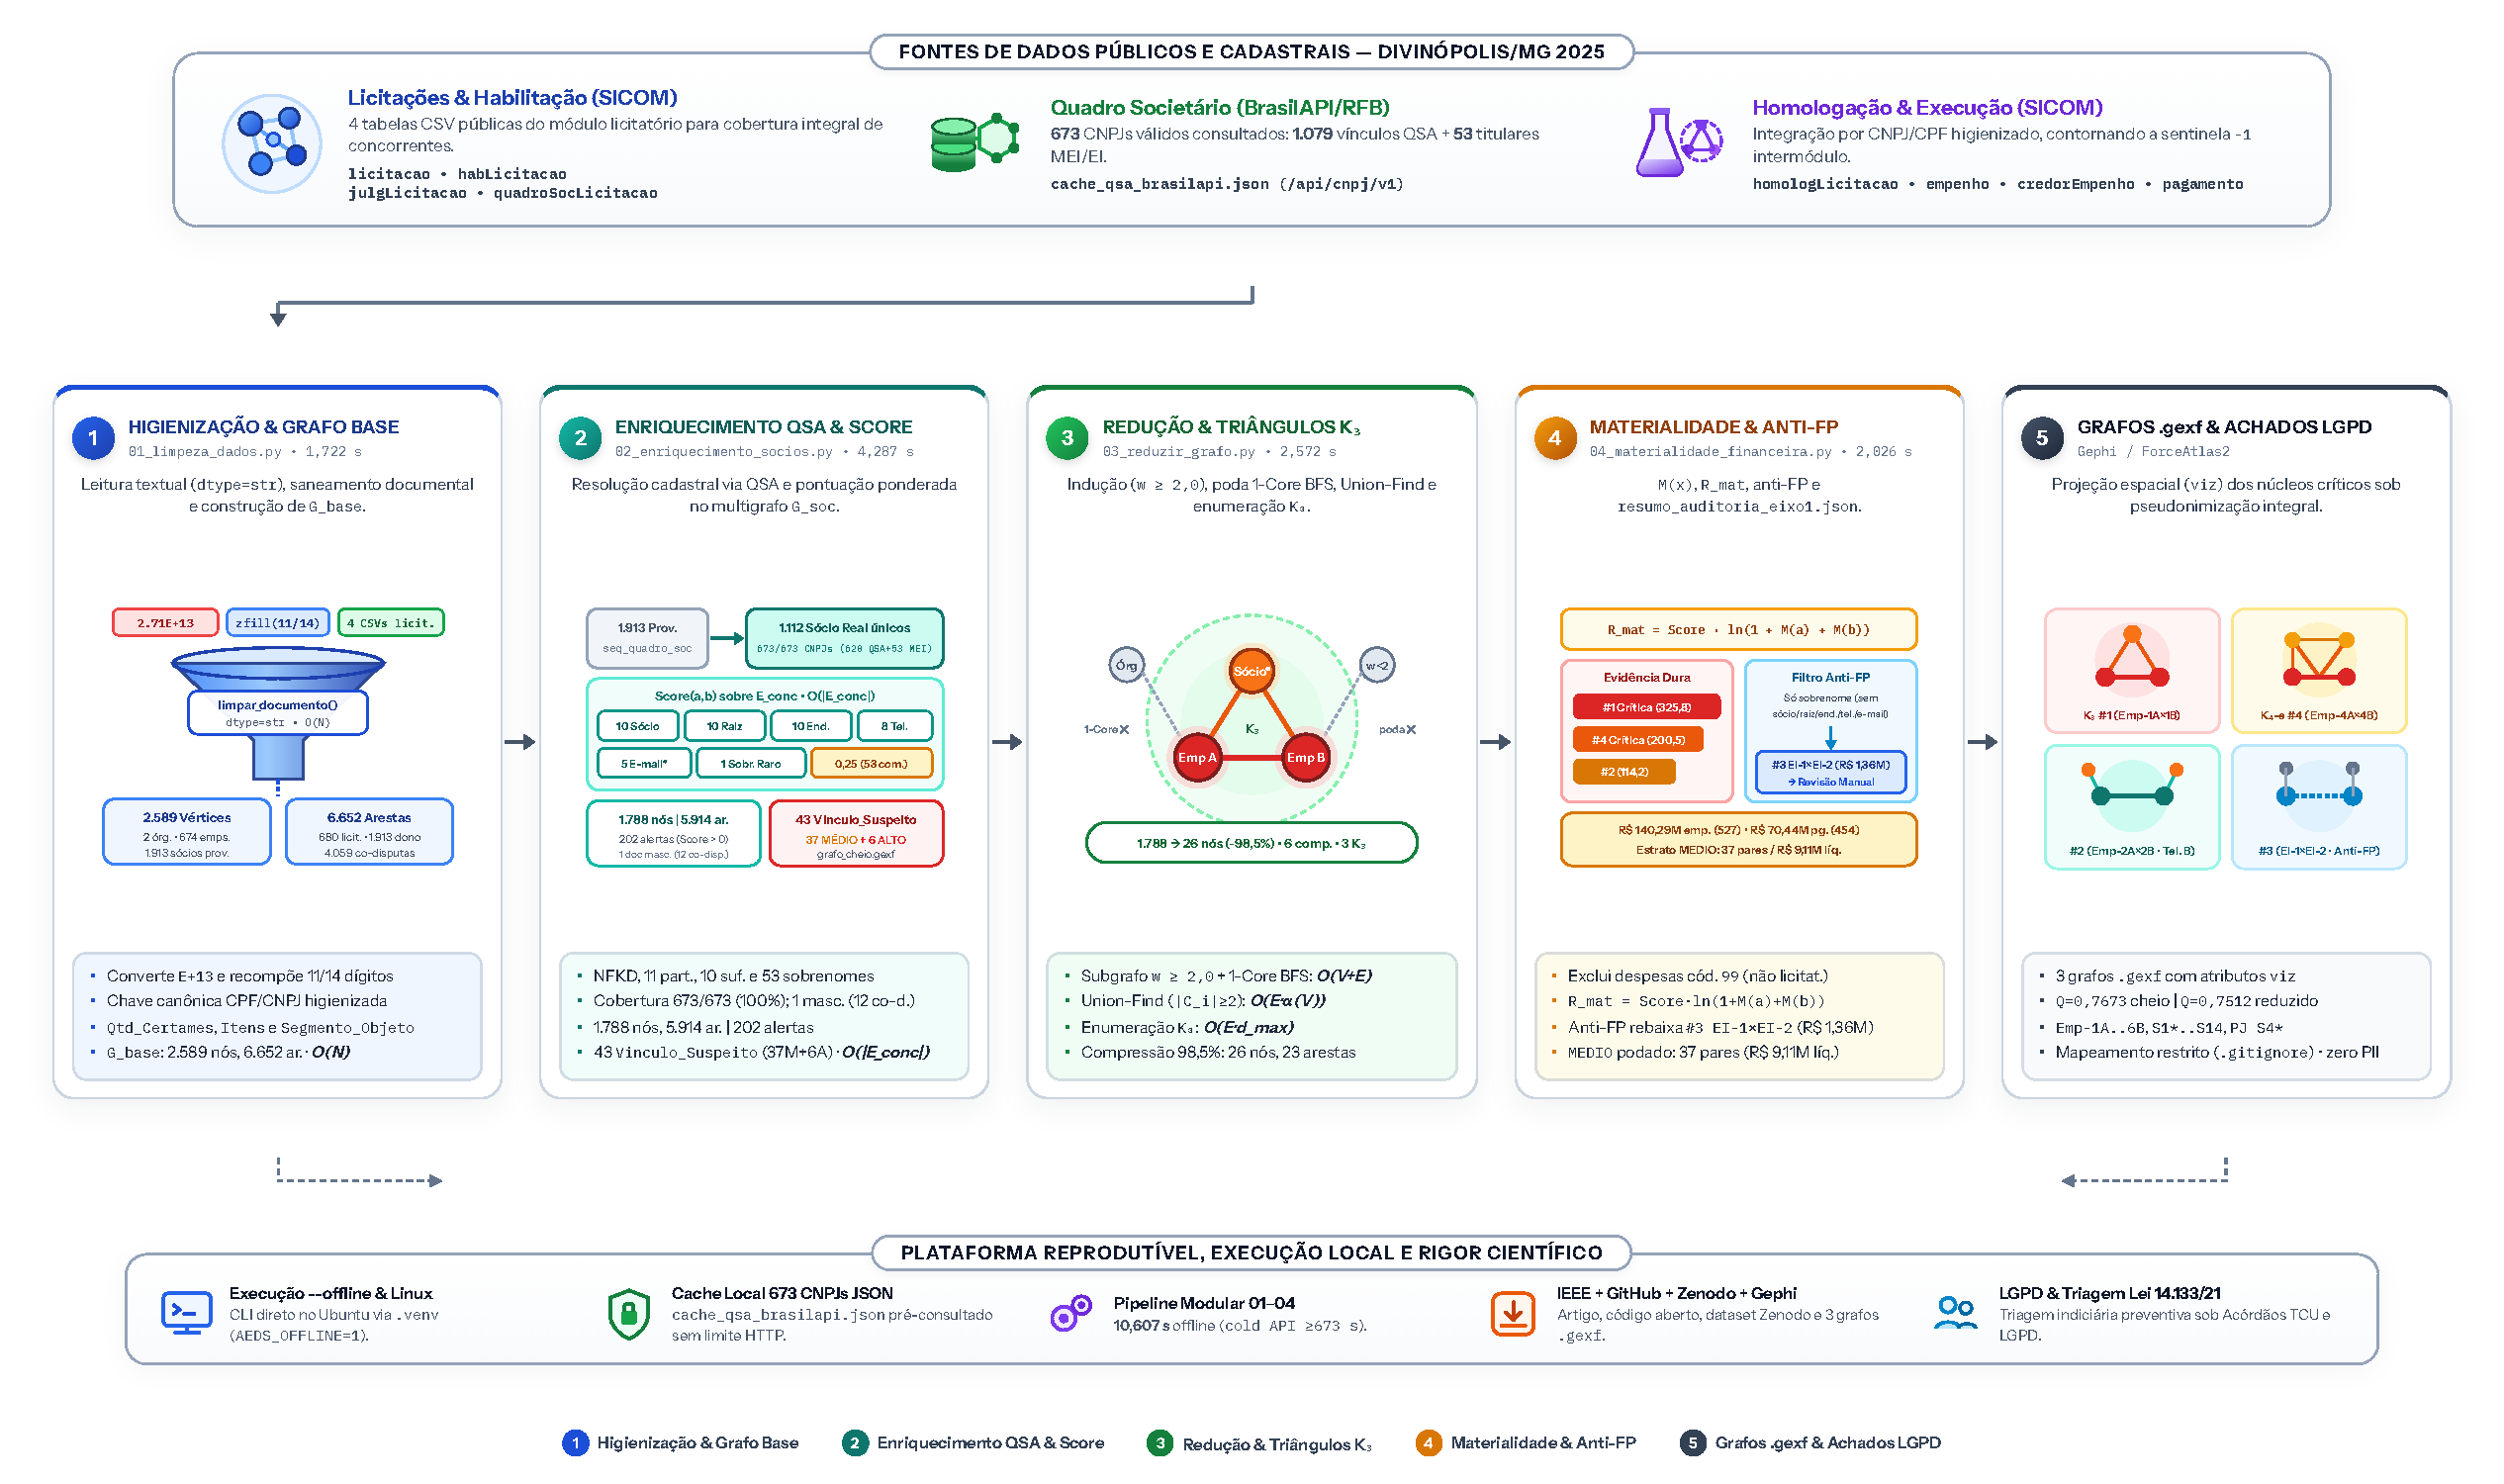
\includegraphics[width=0.93\textwidth]{figures/fluxograma_eixo1.pdf}
\caption{Fluxograma metodológico exclusivo do módulo \texttt{01\_\allowbreak analise\_\allowbreak socios}, organizando a camada superior de fontes públicas e cadastrais (SICOM/TCE-MG 2025 e BrasilAPI/RFB), os cinco blocos operacionais e visuais (1~Higienização \& Grafo Base, 2~Enriquecimento QSA \& Score, 3~Redução \& Triângulos $K_3$, 4~Materialidade \& Anti-FP e 5~Grafos \texttt{.gexf} \& Achados LGPD) com cobertura de 673/673 CNPJs, estrato \texttt{MEDIO} (R\$\,9,11\,M líq.), 10,607\,s em memória e governança LGPD com mapeamento restrito.}
\label{fig:fluxograma_eixo1}
\end{figure*}

\subsection{Obtenção e Tratamento de Dados}

Os registros licitatórios e financeiros provêm das remessas consolidadas de 2025 do município de Divinópolis/MG (código IBGE/SICOM \texttt{3122306}) no Portal de Dados Abertos do TCE-MG~\cite{tce_mg_dados_abertos,tcemg2025in01}. 
Foram processadas quatro tabelas relacionais em CSV delimitados por ponto e vírgula do módulo \texttt{licitacao} (\texttt{licitacao\allowbreak .csv}, \texttt{hab\allowbreak Licitacao\allowbreak .csv}, \texttt{julg\allowbreak Licitacao\allowbreak .csv} e \texttt{quadro\allowbreak Soc\allowbreak Licitacao\allowbreak .csv}) na modelagem estrutural. % além de \texttt{homolog\allowbreak Licitacao\allowbreak .csv}, \texttt{empenho\allowbreak .csv}, \texttt{credor\allowbreak Empenho\allowbreak .csv} e \texttt{pagamento\allowbreak .csv} na etapa de materialidade.

A análise exploratória dos dados revelou um gargalo de integridade na base pública: documentos fiscais (CPF/CNPJ) exportados em planilhas com perda de zeros à esquerda ou notação científica literal (ex.: \texttt{2.71E+13}).  %e (ii) preenchimento sistemático das chaves estrangeiras intermódulo (\texttt{seq\_\allowbreak licitacao} e \texttt{seq\_\allowbreak dispensa}) com o valor sentinela \texttt{-1} nas tabelas de contratos e empenhos, inviabilizando a junção direta entre um certame isolado e seu empenho correspondente. Em contrapartida, as chaves intramódulo (\texttt{seq\_\allowbreak licitacao}, \texttt{seq\_\allowbreak item\_\allowbreak licitacao} e \texttt{seq\_\allowbreak empenho}) preservam integridade completa, permitindo usar o documento fiscal higienizado como chave canônica de integração entre licitações e execução orçamentária.
Aplicou-se uma rotina de saneamento estrutural para corrigir mutações de formatação em notação científica  e restaurar os zeros à esquerda, padronizando 14 dígitos para pessoas jurídicas (CNPJ) e 11 dígitos para pessoas físicas (CPF). Em seguida, consolidoum-se os participantes únicos registrados nas fases de habilitação e julgamento dos certames.

\subsection{Modelagem do Grafo Multicamada}

%A partir da análise exploratória dos dados, todas as tabelas são carregadas em modo estritamente textual (\texttt{dtype=str}). Foram removidas pontuações, converção de expressões em notação científica (\texttt{E+}) para inteiro longo e recompoziação de zeros à esquerda para 11 dígitos (CPF) ou 14 dígitos (CNPJ). Na sequência, construiu-se o grafo base $G_{\text{base}}$:

Após consolidar o conjunto único de licitantes participantes nas fases de habilitação e julgamento, a malha de contratações públicas é formalmente modelada como um grafo heterogêneo multicamada ponderado \begin{equation} G = (V,E,\tau,\phi,w). \end{equation} Nessa formulação, $V$ denota o conjunto global de entidades e $E \subseteq V \times V$ representa o conjunto de interações. A heterogeneidade das entidades é definida pela função de mapeamento $\tau : V \rightarrow \mathcal{T}_V$, enquanto a estrutura multicamada é estabelecida pela função $\phi : E \rightarrow \mathcal{T}_E$, que segrega as relações em quatro camadas sobrepostas. Por fim, a função de ponderação $w : E \rightarrow \mathbb{R}^{+}$ associa a cada aresta uma métrica escalar de intensidade. \subsubsection{Partições de Vértices ($\mathcal{T}_V$)} \begin{itemize} \item \textbf{Órgãos Públicos ($\tau(v)=\text{Órgão}$):} representam as entidades contratantes da administração pública municipal. \item \textbf{Empresas Licitantes ($\tau(v)=\text{Empresa}$):} compreendem os agentes econômicos (pessoas jurídicas e físicas) participantes das fases de habilitação ou julgamento dos certames. \item \textbf{Sócios e Controladores ($\tau(v)=\text{Sócio Real}$):} correspondem aos proprietários e administradores vinculados às empresas licitantes, englobando tanto pessoas físicas (\texttt{PF}) quanto pessoas jurídicas ou \textit{holdings} (\texttt{PJ}). \end{itemize} \subsubsection{Camadas de Arestas ($\mathcal{T}_E$)} \begin{itemize} \item \texttt{Participou\_Licitacao}: camada bipartida que conecta cada \texttt{Empresa} ao respectivo \texttt{Órgão} contratante. \item \texttt{Concorreu\_Contra}: projeção ponderada monopartida entre pares de \texttt{Empresa} que disputaram os mesmos certames, cujo peso acumula a frequência absoluta de licitações e itens individuais disputados em comum. \item \texttt{É\_Dono\_De}: camada bipartida de propriedade que vincula cada \texttt{Sócio Real} às respectivas empresas (\texttt{Empresa}) integrantes de seu quadro societário. \item \texttt{Vinculo\_Suspeito}: camada indiciária filtrada entre pares concorrentes de \texttt{Empresa} que apresentam sobreposição cadastral, societária ou onomástica relevante, ponderada pelo escore de vínculo $w(e)=s(a,b)$. \end{itemize} Embora relações como \texttt{É\_Dono\_De} e \texttt{Participou\_Licitacao} possuam direcionalidade semântica natural, todas as arestas são armazenadas de forma simétrica (não-direcionada) na estrutura computacional em lista de adjacência, viabilizando a poda de grau e a detecção direta de ciclos fechados envolvendo empresas concorrentes e seus controladores em comum.

\subsection{Enriquecimento Societário e Escore Multidimensional de Vínculo} 

Como a tabela societária original do SICOM suprime nomes e CPFs dos sócios por restrição cadastral, executou-se um enriquecimento dos dados mediante consultas automatizadas ao Quadro de Sócios e Administradores (QSA) da Receita Federal via BrasilAPI para os CNPJs licitantes, com persistência em cache local. Para Microempreendedores Individuais (MEIs) e empresários individuais desprovidos de QSA formal, o titular é extraído diretamente da razão social mediante a remoção dos dígitos iniciais do documento. Para evitar falsos positivos decorrentes de dados cadastrais incompletos ou terceirização contábil, aplicam-se filtros determinísticos anti-ruído antes das comparações entre pares: 
\begin{itemize} 
  \item \textbf{Endereços e Telefones:} normalizam-se logradouro, número, município e unidade federativa, descartando entradas genéricas ou sem número e exigindo sequências telefônicas válidas com ao menos oito dígitos. \item \textbf{Correio Eletrônico:} endereços contendo termos associados a escritórios terceirizados (\texttt{contabil}, \texttt{contador}, \texttt{contabilidade}, \texttt{assessoria} e \texttt{escritorio}) são descartados automaticamente. 
  \item \textbf{Onomástica (Sobrenomes):} consideram-se exclusivamente sócios pessoas físicas ou titulares de MEI, removendo o primeiro prenome, preposições conectoras e sufixos de agnação. 
\end{itemize} 
Para atenuar falsos positivos decorrentes de homonímia conuns brasileiras,implementou-se uma ponderação onomástica discreta inspirada no princípio da Frequência Inversa de Documentos (IDF). Cada sobrenome compartilhado $n$ recebe peso reduzido $w(n)=0,25$ quando pertence a um dicionário de sobrenomes triviais, e peso integral $w(n)=1,00$ caso contrário. Para cada par de empresas concorrentes $(a,b)$ conectado na camada \texttt{Concorreu\_Contra}, o escore de vínculo é definido por: \begin{equation} \begin{aligned} s(a,b) =\;& 10 \cdot |S(a)\cap S(b)| \\ & + 10\cdot[\mathrm{raiz}(a)=\mathrm{raiz}(b)] \\ & + 10\cdot[\mathrm{end}(a)=\mathrm{end}(b)] \\ & + 8\cdot[\mathrm{tel}(a)=\mathrm{tel}(b)] \\ & + 5\cdot[\mathrm{email}(a)=\mathrm{email}(b)] \\ & + \sum_{n\in N(a)\cap N(b)} w(n). \end{aligned} \end{equation} onde $S(x)$ denota o conjunto de sócios da empresa $x$, $\mathrm{raiz}(x)$ os oito primeiros dígitos do CNPJ, $\mathrm{end}(x)$, $\mathrm{tel}(x)$ e $\mathrm{email}(x)$ os atributos cadastrais higienizados, e $N(x)$ o conjunto de sobrenomes extraídos. A recorrência acumulada de disputas (\texttt{Peso\_Concorrencia}) não integra a soma de $s(a,b)$, sendo utilizada exclusivamente como critério de desempate na ordenação dos alertas. Os pares com $s(a,b)>0$ são estratificados em três níveis de criticidade: \texttt{ALTO}, quando há identidade direta de sócio, raiz de CNPJ, endereço ou telefone, ou quando $s(a,b)\geq 2,00$; \texttt{MEDIO}, quando $1,00 \leq s(a,b) < 2,00$ sem coincidência cadastral direta; e \texttt{BAIXO}, quando $0 < s(a,b) < 1,00$, sendo estes últimos omitidos da camada indiciária do grafo completo.

\subsection{Redução Topológica e Identificação de Motivos Estruturais ($K_3$)} 
Na rede completa, a elevada centralidade dos órgãos públicos e a densidade da concorrência regular ofuscam as estruturas de conluio. Para isolar os núcleos críticos, aplicou-se uma cadeia sequencial de quatro algoritmos formais em grafos. 
\begin{enumerate} 
\item \textbf{Subgrafo Induzido por Arestas (\textit{Edge-Induced Subgraph}):} Seja $V_{\text{suspeito}}$ o conjunto das empresas incidentes em alguma aresta \texttt{Vinculo\_Suspeito} com peso acima do limiar crítico $\theta = 2,00$. Em varredura linear de complexidade $O(|V|+|E|)$, retêm-se exclusivamente as arestas que satisfazem \begin{equation} \begin{aligned} \mathcal{P}(u,v,\mathrm{tipo},\mathrm{peso}) \iff &\;(\mathrm{tipo}=\texttt{Vinculo\_Suspeito} \\ &\land \mathrm{peso}\geq\theta) \\ &\lor (\mathrm{tipo}=\texttt{É\_Dono\_De} \\ &\land (u\in V_{\text{suspeito}} \lor v\in V_{\text{suspeito}})). \end{aligned} \end{equation} \
\item \textbf{Decomposição 1-Core via BFS:} Utilizando uma fila FIFO (\textit{First-In, First-Out}), executa-se a poda iterativa de grau em complexidade $O(|V|+|E|)$, removendo todos os vértices com grau $d(u)<1$ e preservando exclusivamente os nós ativos no subgrafo reduzido. \item \textbf{Componentes Conexas via Union-Find:} Aplica-se a estrutura de conjuntos disjuntos (\textit{Disjoint Set}) otimizada com \textit{path compression} e \textit{union by rank}, resultando em complexidade quase linear \begin{equation} O(|E| \cdot \alpha(|V|)), \end{equation} onde $\alpha$ representa a função inversa de Ackermann. Retendo apenas componentes não triviais ($|C_i| \geq 2$), a rede é particionada em núcleos independentes de suspeita para auditoria. \item \textbf{Listagem de Triângulos Societários (\textit{Triangle Listing} -- Motivo $K_3$):} Para detectar ciclos fechados de controle econômico compartilhado ($\text{Sócio} - E_1 - E_2 - \text{Sócio}$), constrói-se o mapeamento \begin{equation} \mathrm{donos}[e] = \{s \mid (s,e)\in E_{\texttt{É\_Dono\_De}}\}, \end{equation} e calcula-se a interseção \begin{equation} \mathrm{donos}[e_1]\cap \mathrm{donos}[e_2] \end{equation} para cada aresta suspeita $(e_1,e_2)$ em tempo $O(|E|\cdot d_{\max})$, sendo $d_{\max}$ o número máximo de sócios por empresa. A presença do motivo estrutural $K_3$ formaliza a evidência topológica de ausência de independência decisória entre licitantes formalmente concorrentes. \end{enumerate}

\subsection{Conformidade com a LGPD e Ética em Pesquisa Pública}

Embora as remessas do SICOM/TCE-MG e os dados cadastrais do QSA sejam públicos por determinação legal, a divulgação acadêmica de escores de risco exige proteção proporcional de pessoas naturais e jurídicas conforme a LGPD~\cite{brasil2018lgpd} e os parâmetros do TCU~\cite{tcu2011acordao2341,tcu2024acordao1798}. Em observância à minimização e à adequação de finalidade (art.~6º, incisos~I a III), todo o texto, as tabelas e as figuras aplicam pseudonimização integral: os 14 vértices de sócio dos núcleos reduzidos recebem códigos \texttt{S1*}--\texttt{S14} (sendo \texttt{PJ S4*} uma pessoa jurídica sócia e o sufixo \texttt{*} reservado aos sócios-ponte que fecham triângulos $K_3$), os endereços e telefones coincidentes constam como \texttt{End.~A/B} e \texttt{Tel.~A/B}, as empresas privadas e empresários individuais recebem rótulos \texttt{Emp-1A}--\texttt{Emp-6B} e \texttt{EI-1}--\texttt{EI-2}, e suprimem-se integralmente CPFs, CNPJs e nomes civis. % Para permitir auditoria externa pelas autoridades competentes sem expor dados pessoais no artigo ou no repositório público, a Etapa~4 gera localmente a chave de reversão \texttt{mapeamento\_\allowbreak pseudonimos\_\allowbreak restrito\allowbreak .csv} (30 registros), mantida estritamente offline sob proteção de \texttt{.gitignore}.
